La historia de AFP Capital se remonta a noviembre de 1980, cuando se implementó en Chile el sistema de pensiones de capitalización individual. El 16 de enero de 1981, se constituyó la sociedad Administradora de Fondos de Pensiones Santa María, que más tarde se transformaría en AFP Capital S.A. Desde sus inicios, la empresa se destacó por su filosofía de servicio, enfocada en satisfacer las necesidades y expectativas de sus afiliados. 
En 1995, AFP Capital estableció la filial Santa María Internacional S.A., con el propósito de expandir su alcance y ofrecer servicios a personas naturales o jurídicas del extranjero, así como invertir en AFP o sociedades relacionadas con materias previsionales en otros países. Esta iniciativa consolidó la presencia de AFP Capital en el ámbito internacional y fortaleció su posición como una administradora de fondos de pensiones líder en la región. 
En el año 2000, se produjo una relevante transacción en la historia de AFP Capital. ING Group adquirió Aetna Inc., incluyendo el 96,56\% de las acciones de AFP Capital S.A. Esta adquisición tuvo como objetivo reforzar la posición de liderazgo de AFP Capital en el mercado previsional chileno y contribuir a su crecimiento y desarrollo. 
Posteriormente, en 2008, AFP Capital llevó a cabo una fusión con AFP Bansander, otra reconocida administradora de fondos de pensiones en Chile. Esta fusión permitió consolidar aún más las operaciones de AFP Capital y fortalecer su presencia en el país. A fines de 2011, Grupo SURA, una empresa líder en el negocio de pensiones en Latinoamérica, adquirió las operaciones de ING en la región. Esta adquisición llevó a AFP Capital a formar parte de Grupo SURA y a beneficiarse de su amplia experiencia y recursos, consolidándose como una compañía destacada en el mercado previsional latinoamericano. En resumen, la historia de AFP Capital está marcada por su constante evolución, consolidación y liderazgo en el mercado de administración de fondos de pensiones en Chile. A lo largo de los años, ha demostrado su compromiso con la excelencia en la prestación de servicios previsionales y su capacidad de adaptación a los cambios y desafíos del entorno económico y regulatorio.

\begin{figure}[H]
    \begin{minipage}[t]{0.9\textwidth}
        \caption{Historia AFP Capital}
        \label{historia-afp}        
    \end{minipage}

    \vspace{10pt}

    \begin{minipage}[b]{1.1\textwidth}
        \centering
        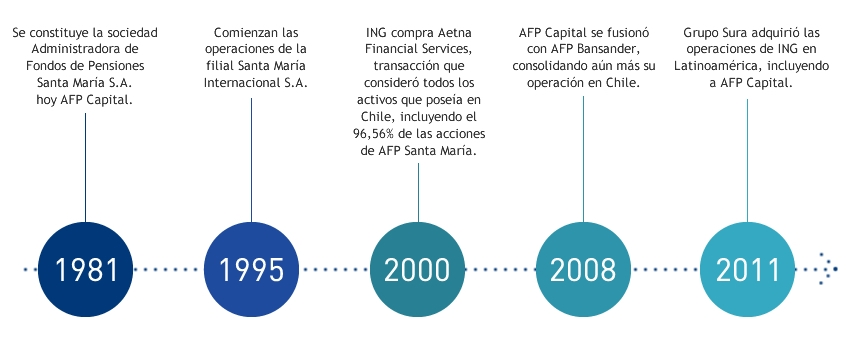
\includegraphics[width=\textwidth]{img/historia-afp-capital.jpg}        
    \end{minipage}

    \begin{minipage}[t]{0.9\textwidth}
        Fuente: AFP Capital. Recuperado de \url{https://www.afpcapital.cl/Quienes-Somos/Paginas/Historia.aspx}
    \end{minipage}
\end{figure}